\iffalse

%-*- program: xelatex -*-        
%-*- program: biber -*-`        
%-*- program: xelatex -*-
\documentclass[12pt]{article}
\usepackage{amsmath,textcomp,amssymb,geometry,graphicx,enumerate,upquote,color}
\usepackage{hyperref}
\usepackage{float}
\usepackage{tikz}
\usepackage{array}
\usepackage{amsfonts}
\def\Session{Fall 2015}
\usepackage[english]{babel}
\title{Relationship between Serial Correlation and Different Risk Measurement}
\author{Boying Gong, Xinyue Zhou}
\newenvironment{qparts}{\begin{enumerate}[{(}a{)}]}{\end{enumerate}}
\def\endproofmark{$\Box$}
\newenvironment{proof}{\par{\bf Proof}:}{\endproofmark\smallskip}
\begin{document}
\maketitle

\fi

\subsection{Explortary Step}
In this section, we have tried to explore the relationship between serial correlation with VaR, ES and CED using several simple time series model. They are AR(1), MA(1) and ARMA(1,1). The three models here are not necessary the best one, or even the ones that all underlying assumptions are satisfied. This step is just try to have a general idea if the serial correlation of each model is related with risk measurements in some way. When it comes to serial correlation here, it refers to the first order autocorrelation of the time series models. 

\subsubsection{AR(1)}

\begin{equation}
X_t = \phi X_{t-1} + \epsilon_t
\end{equation}

AR(1) is the time series model utilized in the paper ON A CONVEX MEASURE OF DRAWDOWN RISK for exploring the relationship between serial correlation and CED of US Equity and US Government Bonds. Here we were trying to implement the same method but expand it to more assets (the eleven US equities). Moreover, we added scatter plots between $\kappa$ and other risk measurements, which enable us to check if CED is more correlated with serial correlation of returns.

Figure \ref{fig:SerCol-VaR5yrAR1}, Figure \ref{fig:SerCol-ES5yrAR1} and Figure \ref{fig:SerCol-CED5yr3monAR1} show the relationship between the theoretical first-order serial correlation and VaR, ES, CED, separately. We can see that the correlation between first-order serial correlation and various risk measures are not so obvious. There are both positive (such as RMZ, BCOM, RAY, USGG10YR) and negative correlations (such as HYG, TIP). The correlation between first-order serial correlation ($\kappa(1)$) and various risk measures are listed in Table \ref{table:corSerialRisk}. We can see from the results that assets such as AGG (0.92) and RMZ (0.90) show high positive correlations, while HYG and TIP show signifiant negative correlation. Moreover, the correlations between VaR ,ES and $\kappa(1)$ are generally greater than the correlation between VaR and $\kappa(1)$.

The Table \ref{table:corSerialRisk} is got from computing the correlation of $\kappa(1)$ and the risk measurement, VaR, ES and CED, which are calculated from the previous study. We also adjust the them to be in the same time period. The time window used for get risk measurements and $\kappa(1)$ is 5 years, and the rolling window within 5 year for CED is 3 month. Consistent with what was showing in the plot, all the assets except MXEA and MXEF have the high correlation between $\kappa(1)$ and risk measurements. Within each asset, as expected, the correlation with VaR and ES are very closed, as VaR is highly correlated with ES internally. However, compared with VaR and ES, the correlation with CED is relatively smaller, and sometimes the correlations are even with different sign. For example, for MXEF asset, the correlation with VaR and ES are positive, and though small, the correlation with CED is negative.

\begin{table}[!h]
\caption{Correlation between $\kappa(1)$ (calculated using AR(1)) and risk measures}
\centering 
\begin{tabular}{ | c || r r r| } 
 \hline
Asset & VaR  & ES & CED \\
  \hline \hline
AGG & 0.92 & 0.95 & 0.94 \\ 
HYG & -0.61 & -0.56 &  -0.41 \\ 
TIP & -0.67 & -0.75 &  -0.73 \\ 
BCOM & 0.86 & 0.80 & 0.76 \\ 
MXEA & 0.26 & 0.33 & 0.08 \\ 
MXEF & 0.23 & 0.22 & -0.05 \\ 
RAY & 0.79 & 0.76 & 0.49 \\ 
RMZ & 0.90 & 0.93 &  0.81 \\ 
SPX & 0.62 & 0.70 & 0.15 \\ 
USGG10YR & 0.67 & 0.64 &  0.66 \\
 \hline
\end{tabular}
\label{table:corSerialRisk}
\end{table}

\iffalse

\begin{figure}
  \caption{First-order serial correlation calculated using AR(1) model versus VaR}
  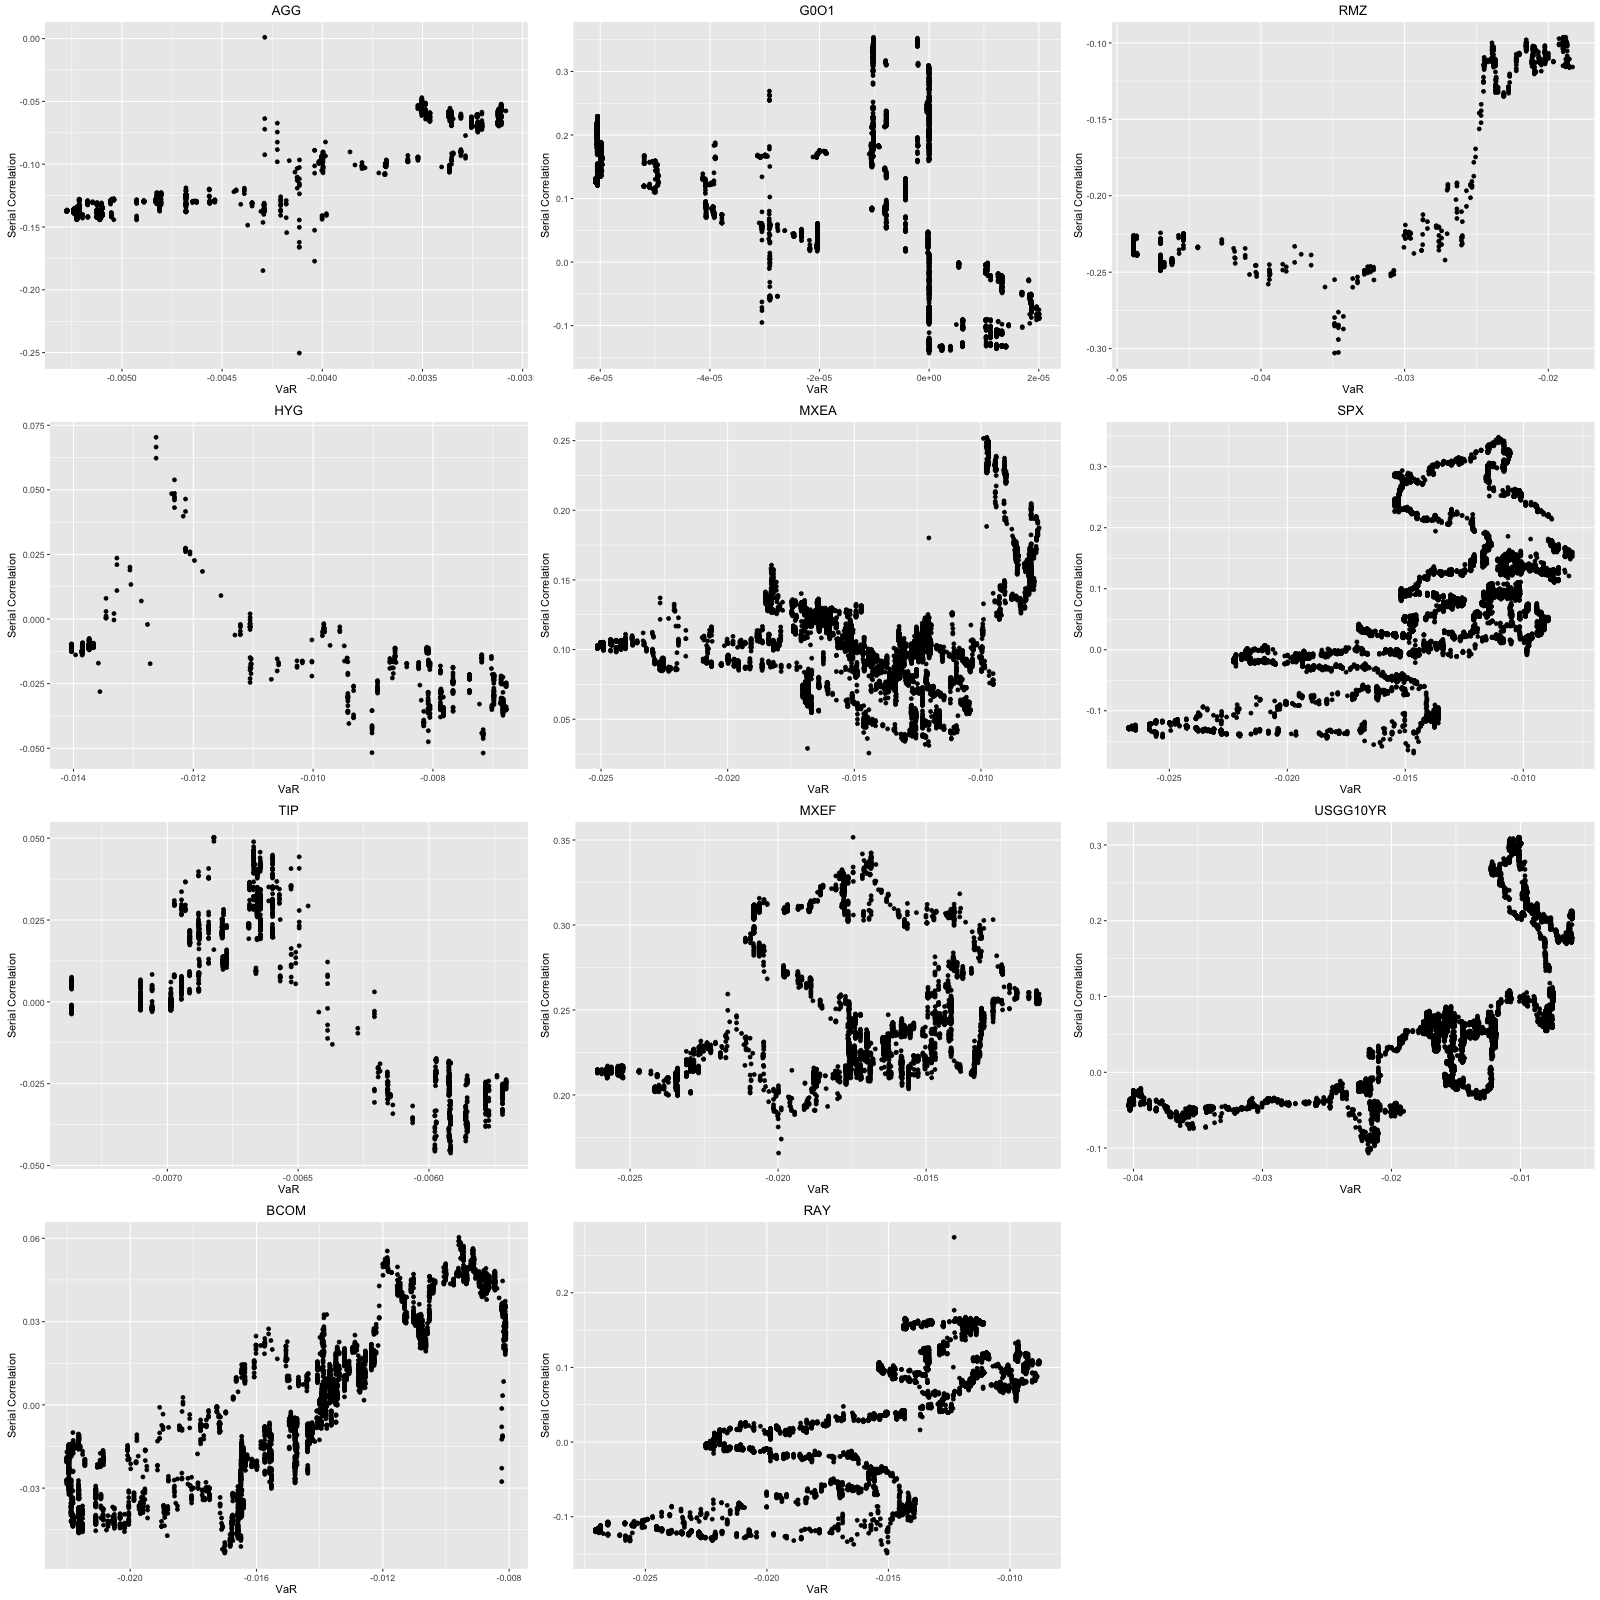
\includegraphics[width = 1\textwidth]{../results/SerCol-VaR5yrAR1}
  \label{fig:SerCol-VaR5yrAR1}
\end{figure}

\begin{figure}
  \caption{First-order serial correlation calculated using AR(1) model versus ES}
  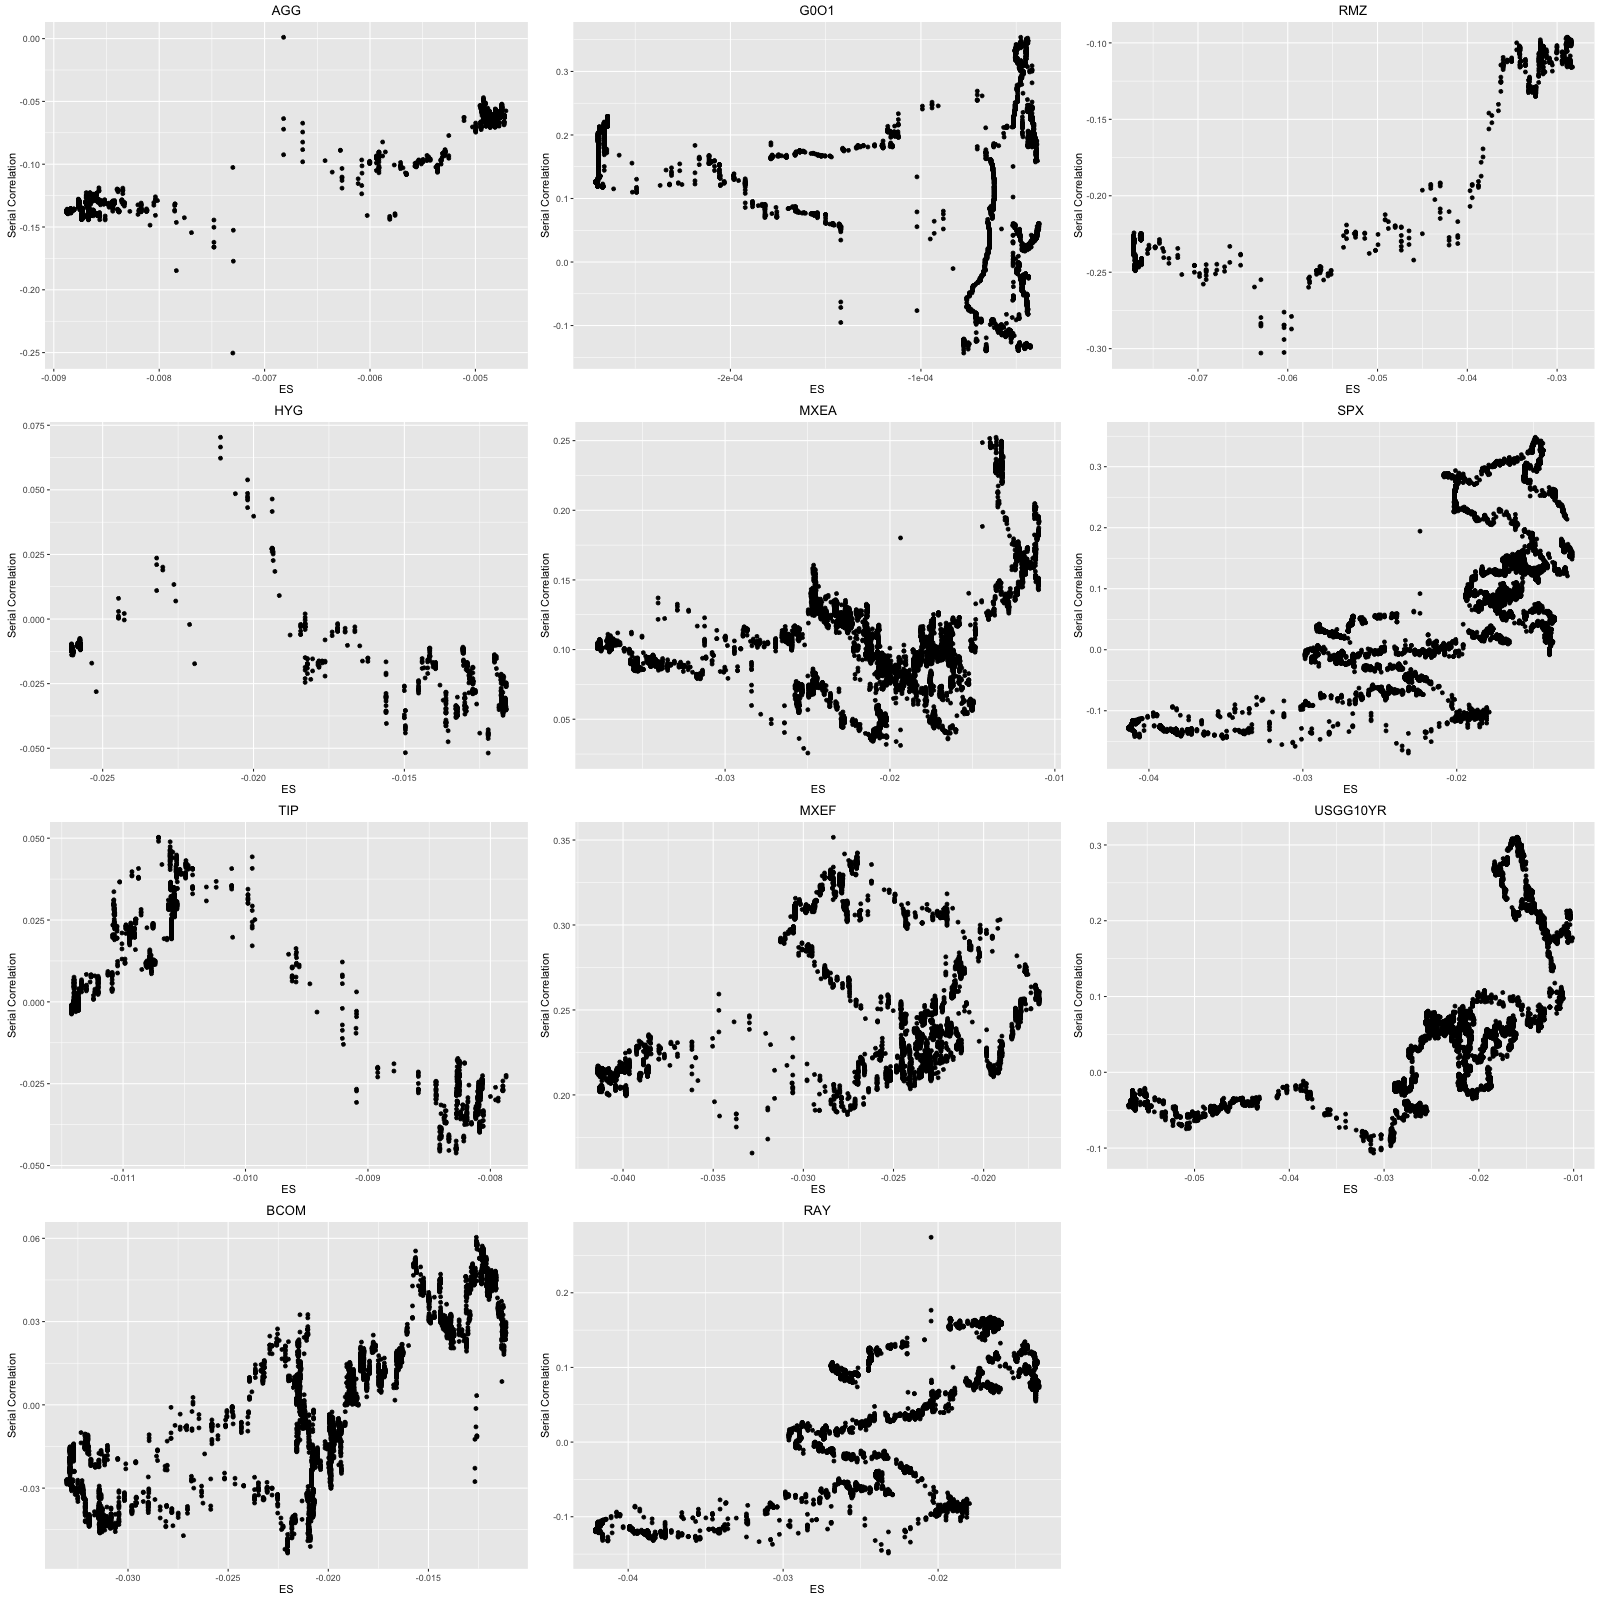
\includegraphics[width = 1\textwidth]{../results/SerCol-ES5yrAR1}
  \label{fig:SerCol-ES5yrAR1}
\end{figure}

\begin{figure}
  \caption{First-order serial correlation calculated using AR(1) model versus CED}
  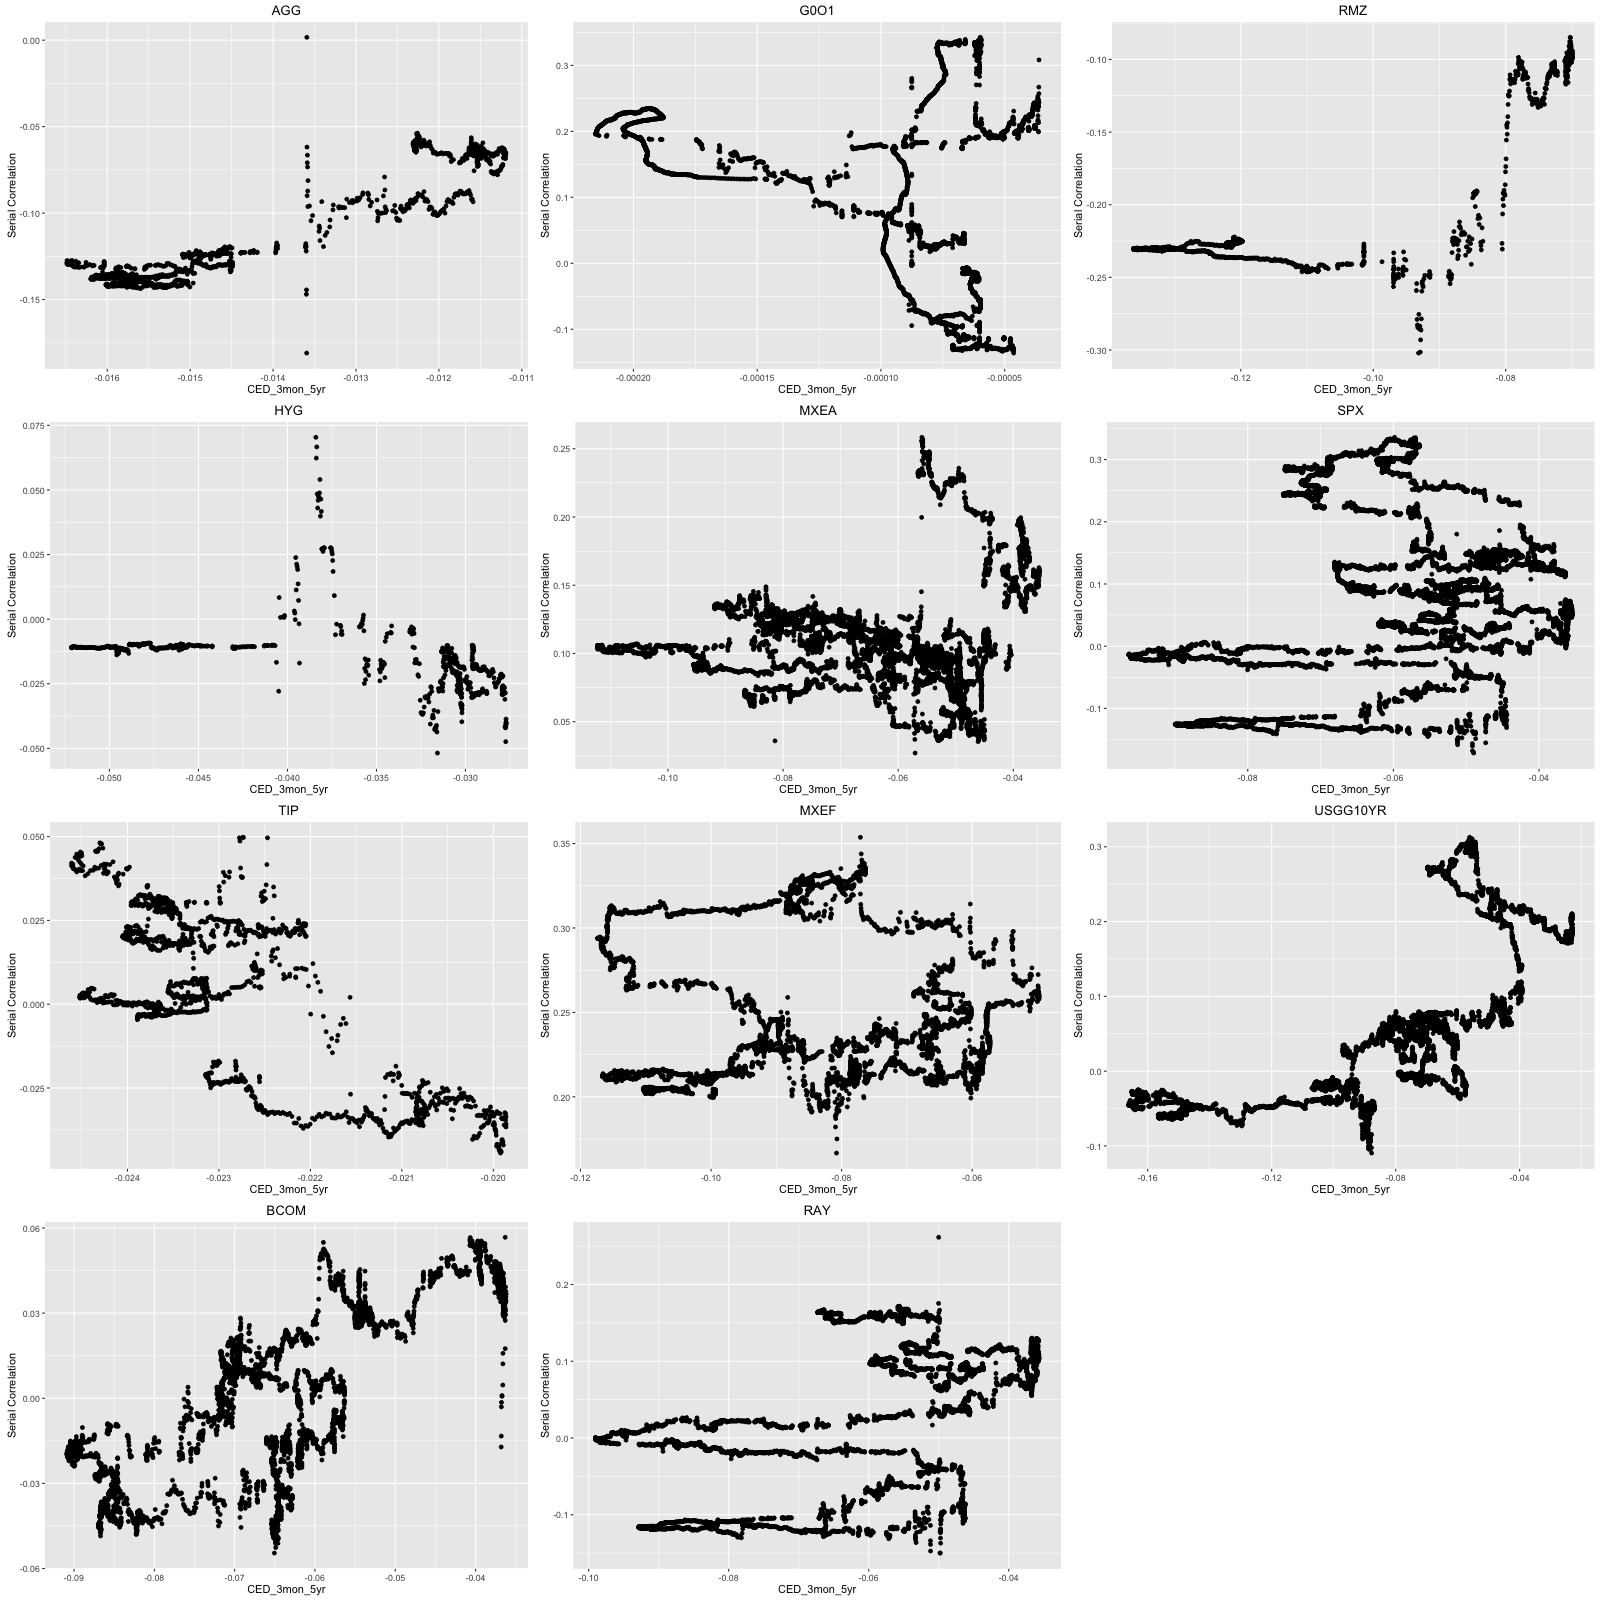
\includegraphics[width = 1\textwidth]{../results/SerCol-CED5yr3monAR1}
  \label{fig:SerCol-CED5yr3monAR1}
\end{figure}

\fi


\subsubsection{MA(1)}
MA(1) is another simple model that is widely used on the Financial time series. In fact, it is a very good one for fitting index \textbf{RMZ}, which will be further elaborated in next section. Since the plot of $\kappa$ vs ES is similar to that with VaR, so only one plot is chosen to put on the report.
\begin{equation}
X_t = \epsilon_t + \theta\epsilon_{t-1}
\end{equation}
For MA(1), there is a simple formula for calculating theoretical first-order serial correlation.
\begin{equation}
\kappa(h) = \begin{cases} \frac{\theta}{(1+\theta^2)} &\mbox{if } h = 1 \\ 
0 & \mbox{otherwise } \end{cases}
\end{equation}

The plots are very similar with that of AR(1) 

\iffalse

\begin{figure}
  \caption{First-order serial correlation calculated using MA(1) model versus VaR}
  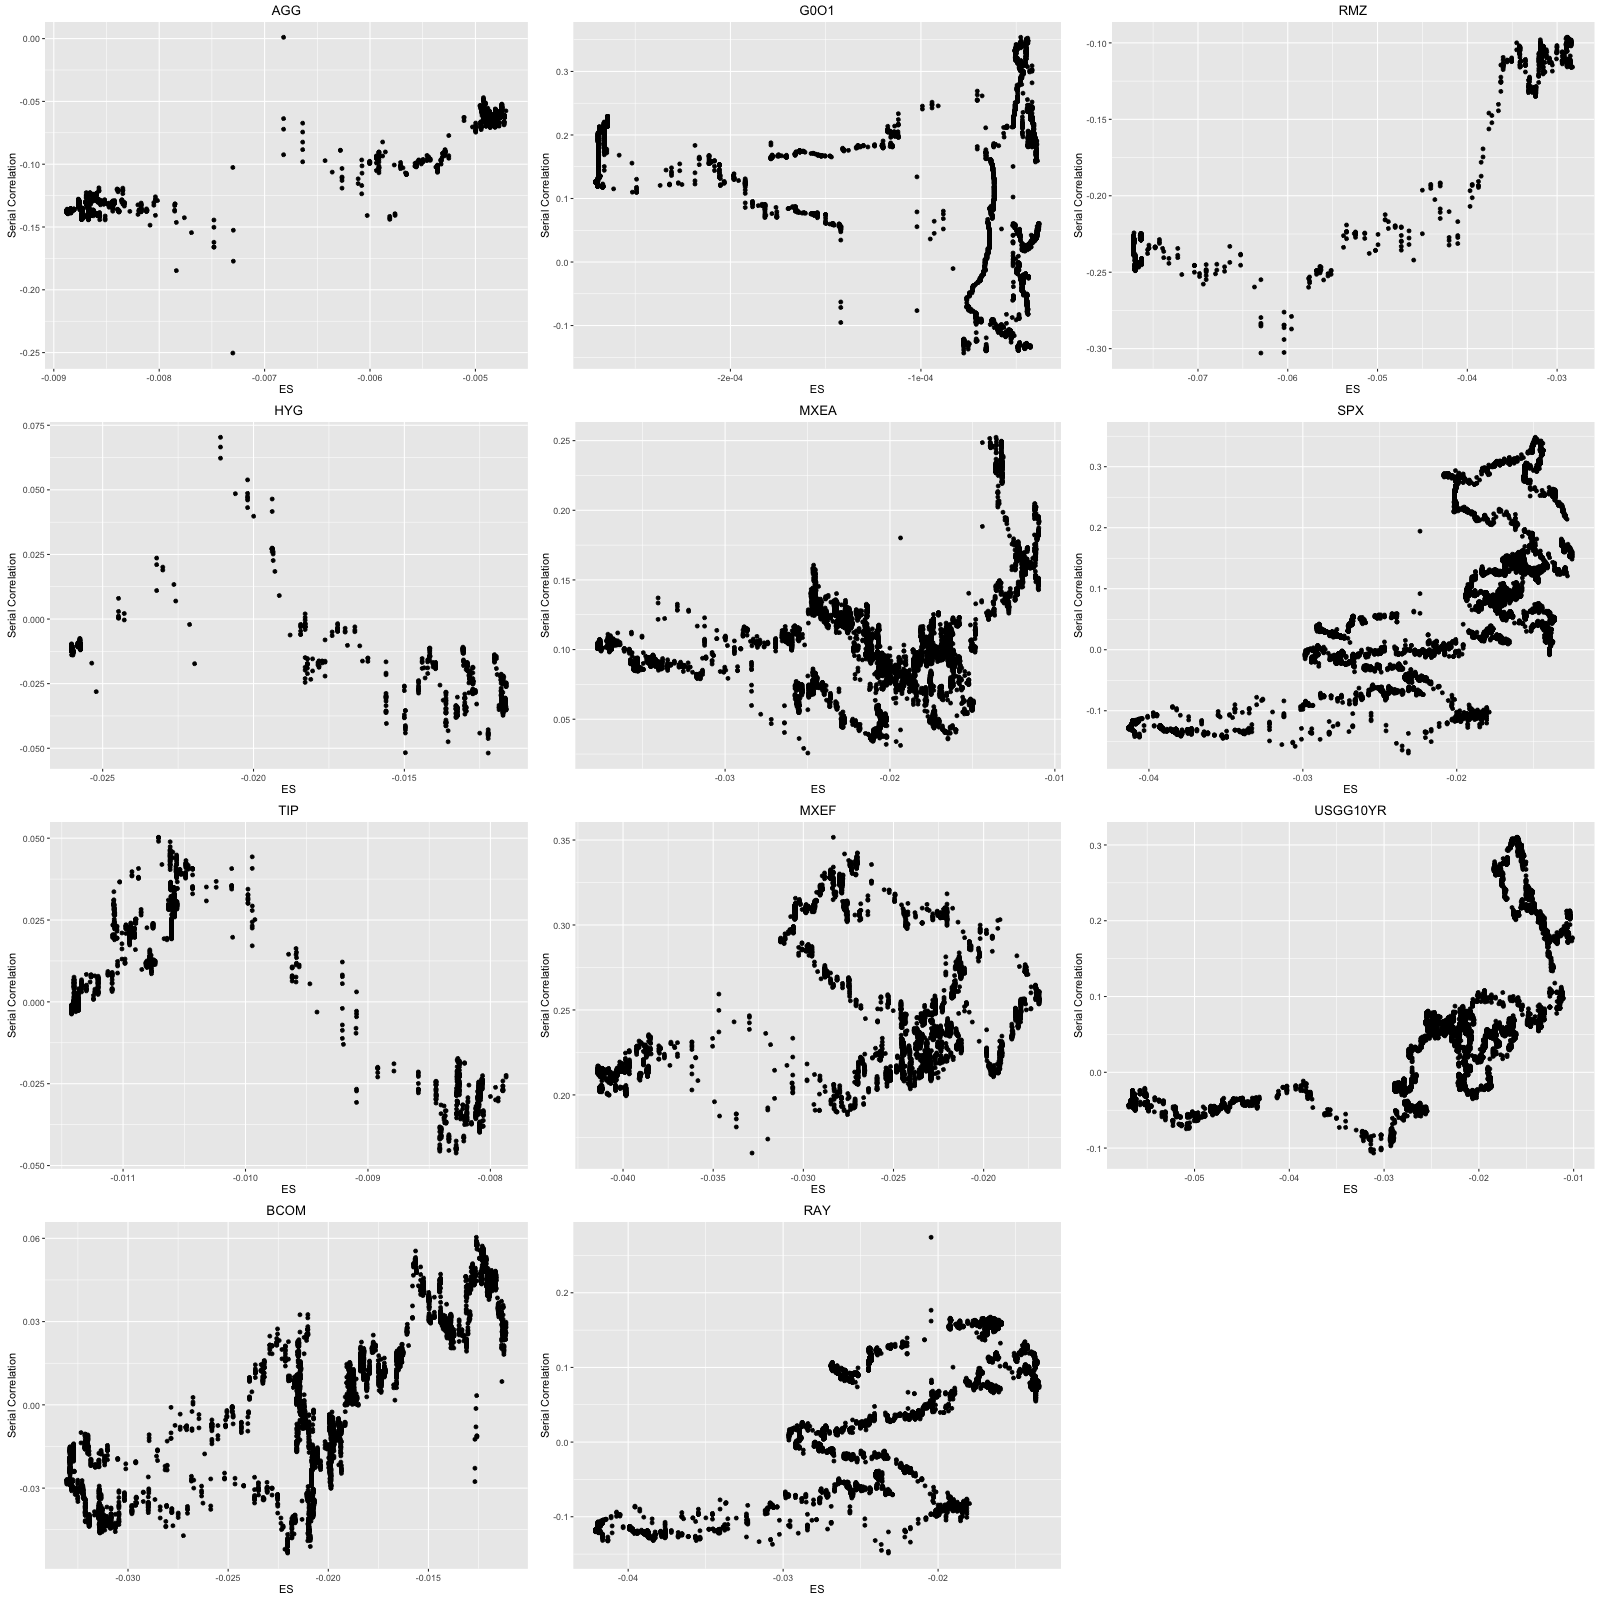
\includegraphics[width = 1\textwidth]{../results/SerCol-ES5yrMA1}
  \label{fig:SerCol-ES5yrMA1}
\end{figure}

\begin{figure}
  \caption{First-order serial correlation calculated using MA(1) model versus CED}
  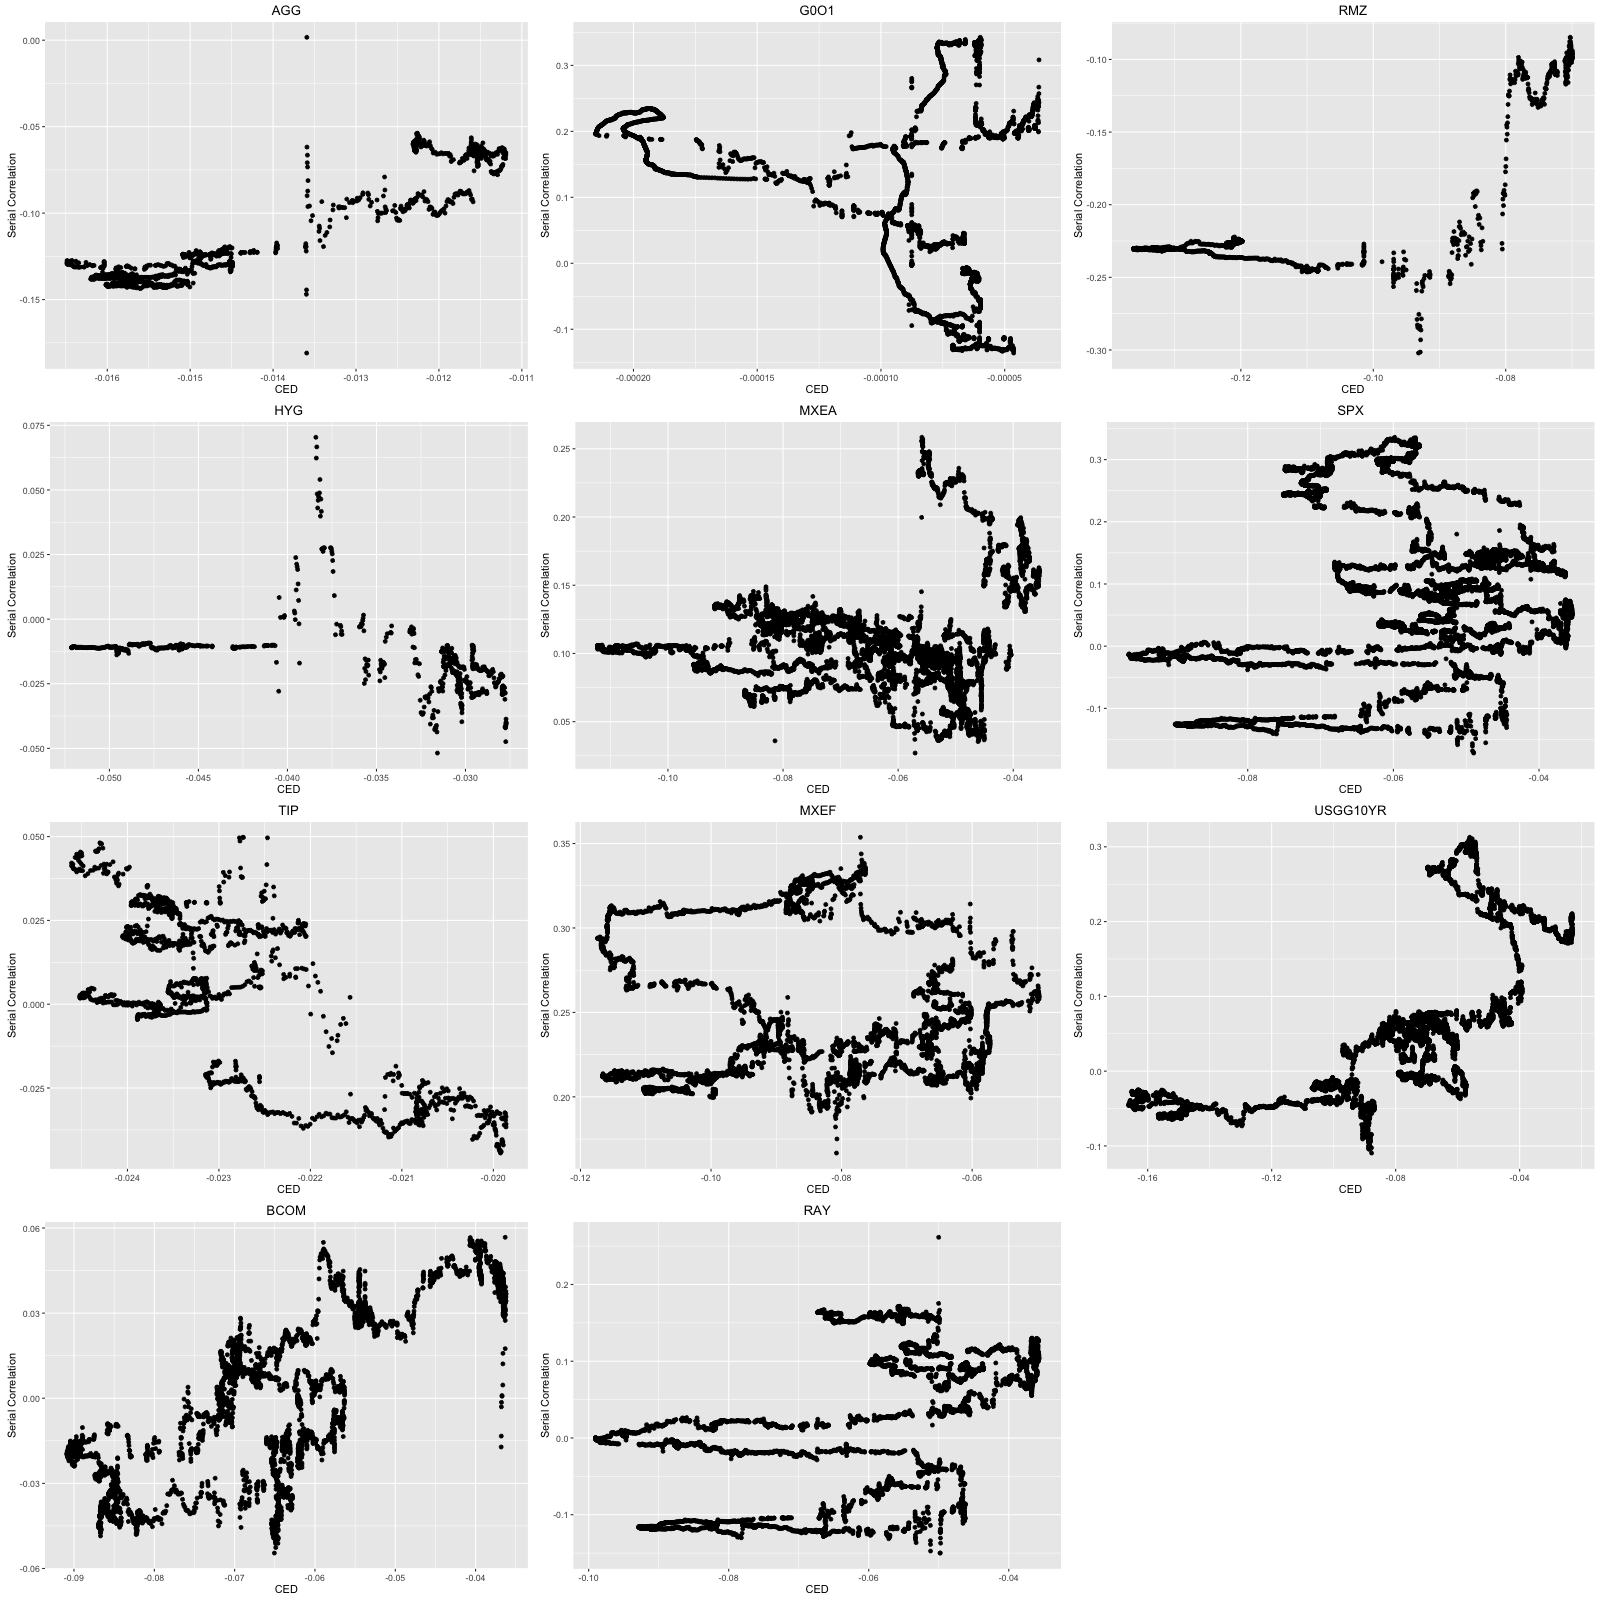
\includegraphics[width = 1\textwidth]{../results/SerCol-CED5yr3monMA1}
  \label{fig:SerCol-CED5yr3monMA1}
\end{figure}

\fi

\begin{table}[!h]
\caption{Correlation between $\kappa(1)$ (calculated using MA(1)) and risk measures}
\centering 
\begin{tabular}{ | c || r r r| } 
 \hline
Asset & VaR  & ES & CED \\
  \hline \hline
AGG & 0.94 & 0.96 & 0.94 \\ 
HYG & -0.51 & -0.45 &  -0.29 \\ 
TIP & -0.65 & -0.74 &  -0.73 \\ 
BCOM & 0.86 & 0.80 & 0.76 \\ 
MXEA & 0.01 & 0.11 & 0.15 \\ 
MXEF & 0.15 & 0.16 & -0.12 \\ 
RAY & 0.79 & 0.77 & 0.50 \\ 
RMZ & 0.92 & 0.95 &  0.84 \\ 
SPX & 0.65 & 0.72 & 0.17 \\ 
USGG10YR & 0.65 & 0.64 &  0.68 \\
 \hline
\end{tabular}
\label{table:corSerialRisk2}
\end{table}

\subsubsection{ARMA(1,1)}

The ARMA(1, 1) has the following expression:

\begin{equation}
X_t = \phi X_{t-1} + \epsilon_t + \theta\epsilon_{t-1}
\end{equation}

The serial correlation calculated using the theoretical expression of fitted ARMA model has a more vague correlation with the various risk measures. The convergence problem occured when fitting the model also indicate a potential model specification.

There is also a formula for calculating the first order correlation for ARMA(1,1) model.
\begin{equation}
\kappa(h) = \frac{(1+\theta \phi)(\theta + \phi)}{1+ 2\theta \phi +\phi^2} \phi^{h-1}, \mbox{if } h \geq 1
\end{equation}

Figure \ref{fig:SerCol-CED5yr3monARMA1} shows the scatter plot of first-order serial correlation calculated using ARMA(1) model versus CED.

\iffalse

\begin{figure}
  \caption{First-order serial correlation calculated using ARMA(1) model versus CED}
  
\includegraphics[width = 1\textwidth]{../results/SerCol-CED5yr3monARMA11}
  \label{fig:SerCol-CED5yr3monARMA1}
\end{figure}

\fi

\subsection{Model Selection}
Things are becoming tricky when it comes to the model selection part. For the fact that it makes no sense to fit different model for each rolling time period within one asset, we tried to find a proper time series model for the all data for each asset. Unfortunately, observing from the ACF plot of returns, they are not stationary by nature without drift term, which means ARMA model is not a good selection for fitting them. It may also explain the reason why the previous section did not produce a expected result that CED is more correlated with serial correlation $\kappa(1)$.

Our criterion here for "better model" is the smaller AIC value. To confirm the fact that ARMA is not reasonable for almost all the indices, we tried sets of parameter for ARMA and select the one with the smallest AIC value. Basically, we chose the combination of AR and MA parameters ranging from 1 to 5.  Here is the results.

AIC short for Akaike information criterion, which is one of the most commonly used criterion for model selection. Here is the formula for AIC.
\[
AIC = 2k - ln(L)
\]
k is the number of parameter in the model and L is the maximum value of the likelihood function for a certain model. Intuitively, AIC rewards goodness of fit (as assessed by the likelihood function), but it also includes a penalty that is an increasing function of the number of estimated parameters \footnote{https://en.wikipedia.org/wiki/Akaike\_information\_criterion}. Therefore, we want the model with smallest AIC value.

\begin{table}[!h]
\caption{Best ARMA Model Based on AIC Value}
\centering 
\begin{tabular}{ | c || r | } 
 \hline
Asset & ARMA (p,q) \\
  \hline \hline
AGG & (5,5)\\ 
HYG & (5,5) \\ 
TIP & (5,4)  \\ 
BCOM & (4,4) \\ 
MXEA & (5,5)  \\ 
MXEF & (5,4) \\ 
RAY & (4,5)  \\ 
RMZ & (3,3)  \\ 
SPX & (5,4) \\ 
USGG10YR & (5,5) \\
 \hline
\end{tabular}
\label{table:bestArmaModel}
\end{table}

From the Table \ref{table:bestArmaModel} almost all the assets, the parameters are as high as 4 or 5, which indicates the time series are not stationary. It also involved some converging issue is when the parameters are getting larger.

For the next step of exploring reasonable model for those assets, several potential models is there can be taken in to consideration:
\begin{itemize}
\item \textbf{ARIMA model with $d=1$}. We found the time series became much more stationary after first-order differencing. 
\item \textbf{ARCH/GARCH model}. Those are the models widely used for financial assets, in which variance of time series are more likely clustering.
\end{itemize}

\subsubsection{EXAMPLE: RMZ data}
Let us take RMZ for example. There are several reasons why we chose to use RMZ: 1) the RMZ has a shorter period, which means a smaller data set to test different time series models. 2) Larger serial correlation and ES, VaR comparing with other indices, implying it is more suitable for analysing the relationship between serial correlation and various risk measures. 3) There are less modes in Maximum drawdown of RMZ, indicating it is reasonable to get tail mean, which is CED.

We also compared RMZ with other index in models selection. From the ACF/PACF plots, RMZ seems the one most suitable for fit ARMA model. Others are not stationary even after a long lag.

First of all, we checked if the time series was stationary in long term. Here is the ACF/PACF plot of the ten-year data. It turns out to be good for using ARMA(0,0,1), MA(1) or ARMA(1,0,1) model, except several lags are a little bit higher than blue line ($|h|$ = 0.05). We also took the first-order difference of the data. The time series become more stationary then before and ARIMA(0,1,1) seems to be a good model for it.

\begin{figure}
  \caption{ACF/PACF of Return for RMZ}
  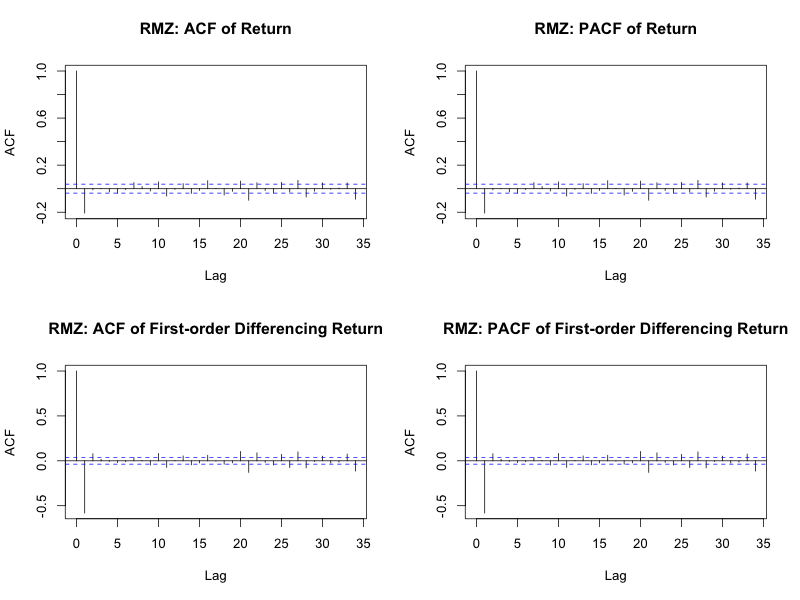
\includegraphics[width = 1\textwidth]{../results/ACFofRMZ}
  \label{fig:ACFofRMZ}
\end{figure}

We also fitted in short time period (1 year period), and the time series became more stationary in each subperiods, and thus the three models mentioned seemed to be reasonable. Below we summarized the model we used for RMZ. We found that the MA(1) model has the smallest AIC within the three parameter sets we chose below. 
\begin{itemize}
\item AR(1) --- to be consistent with your paper
\item MA(1) --- produce least AIC among list 4 models when fitting the all data of RMZ
\item ARMA(1,1)
\item ARIMA(0,1,1) --- Last two is chosen from the pattern of ACF, PACF plot.
\end{itemize}

Here are some diagnostics for MA(1):
\begin{figure}
  \caption{Diagnostic Plots of MA(1) for RMZ}
  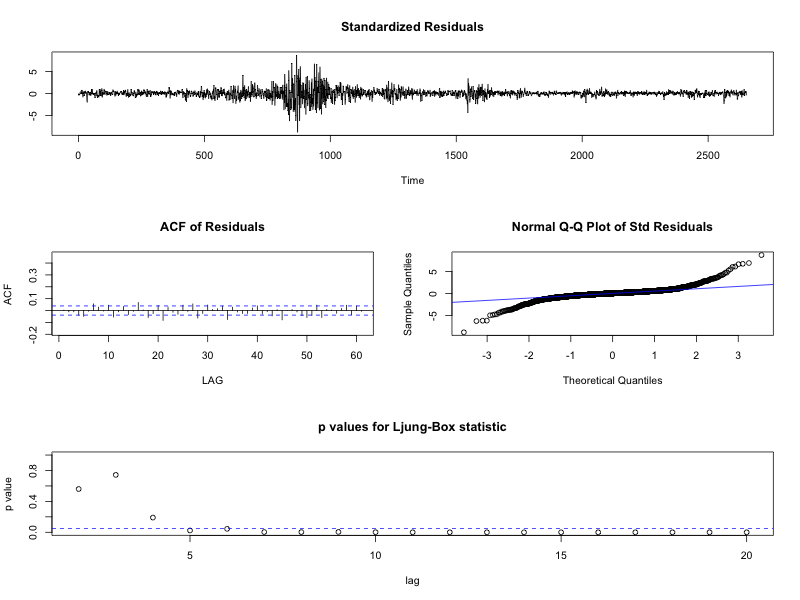
\includegraphics[width = 1\textwidth]{../results/DiagnosticRMZ}
  \label{fig:DiagnosticRMZ}
\end{figure}

From the Figure: \ref{fig:DiagnosticRMZ} above, it is not surprising to see that MA(1) cannot capture the variance cluster in the return, resulting in some variance cluster left the residual plot. There still exists some correlation between residuals after more than 50 lags, but they are comparatively small after the fitting. Normal Q-Q shows that residuals are heavy-tailed. Ljung–Box–Pierce Q-statistic, used for test grouped $\kappa_e(h)$, rejects $H_0$ after $5^{th}$ lag, which also indicates the residual is not white noise after fitting.

In summary, although MA(1) seems to be the good model we could find in ARMA family, it is not enough to capture all the characters in the RMZ return.

\iffalse

\section{Summary: questions}

\subsection{How to find the serial correlation?}

In the paper ON A CONVEX MEASURE OF DRAWDOWN RISK, you fitted the AR(1) model and using the kappa to measure the serial correlation. Now we fit higher order time series model and obtained more than one value of time series coefficient. It's not that reasonable to plot every coefficient versus the risk diagnostics. One solution we came up with is to plot the risk diagnostics versus the serial correlation instead of the time series coefficients. Then how to find serial correlation? 
There are two ways to calculate the serial correlation:
\begin{enumerate}
\item Calculate directly using the return data. For example, for first order serial correlation, we can use $E[X_t X_{t-1}]$;
\item Calculate using the fitted ARMA model. Since we can get the order and coefficients using the fitted model, we may also use them to calculate the theoretical autocorrelation function based on the time series expressions.
\end{enumerate}

We've calculated the serial correlation using both methods, but which one is more reasonable? If the first one is enough, why are we fitting time series model?

\subsection{The correlation between CED and serial correlation is small}

We are supposed to plot the serial correlation verses various risk measure, eg. ES, CED, VaR.  The assumption would be CED is more sensitive to the change of serial correlation, is that right? (And basically we are looking at first order serial correlaion)

We calculated the correlation between first order serial correlation and various risk diagnostics. Then found out they are not that correlated. (with both negative and positive values, compared with the high correlation between various diagnostics which are usually greater than 0.85) Mover, the correlations between serial correlation and CED are even smaller than the correlations between serial correlation and other risk measure. (See Table \ref{table:corSerialRisk})

\subsection{Time series model selection}
 
First, I am curious about the criterion you chose AR(1) for fitting the model in the paper. Is that a common method which is applied to all assets? For our case, when faced more assets with varied property, which criterion are we suppose to use?(right now we use AIC  for model selection). Moreover, when we select the model based on rolling fitting performance, how to choose the criterion? Can we choose to use average AIC, while we think the assumption of using average AIC is the independence between models, which is highly suspicious.


% \bibliographystyle{unsrt}
% \bibliography{analysis}

\end{document}

\fi
